\section{Analysis 3: Spatial Evidence in Language and in Frozen Models}

\paragraph{Motivation and hypotheses.} Idea 5 supplies explicit geometry (depth, segmentation, pose) for norm reasoning. We test two of its premises without training. \textbf{H1}: spatial content is concentrated in a subset of norm categories and is visible in the answer language. \textbf{H2}: geometry maps give a frozen model usable information beyond the RGB frames they are derived from.

\paragraph{Data and protocol.} \emph{Language.} For all 1{,}853 EgoNormia items \citep{rezaei2025egonormia} we embed each action--justification option with mean-pooled \texttt{bert-base-uncased} and compare it with Empath categories and a fixed list of spatial terms, using logistic probes with folds grouped by source video. \emph{Models.} From the released 200-item verified split we keep one item per source video and take the 60 with the sharpest frames, a choice based on image quality alone. Six frozen models answer each item from (i) the answer options only, (ii) the options plus five pre-action RGB frames, and (iii) those plus estimated depth (Depth Anything V2) and instance segmentation (YOLOv8n-seg) of the same frames. Each answer is a separate call with no shared context and counts only if action and justification are both correct.

\begin{figure}[t]
\centering
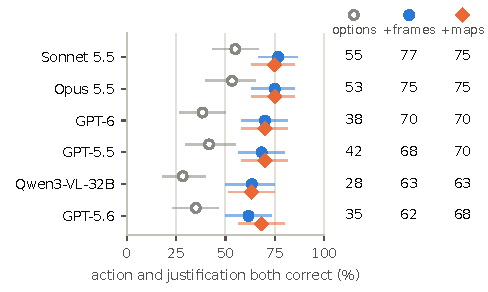
\includegraphics[width=\columnwidth]{analysis3_figure.pdf}
\caption{Joint accuracy of six frozen models on 60 items given the answer options only (grey), plus five RGB frames (blue), and plus depth and segmentation maps of those frames (orange). Lines are 95\% bootstrap intervals.}
\label{fig:a3}
\end{figure}

\paragraph{Results.} \emph{H1.} A spatial term appears in 24.6\% of correct options, most often for Privacy (39.5\%) and Proxemics (33.4\%) and least for Cooperation (20.9\%). Proxemics membership is predicted from text with AUC 0.70 by BERT, against 0.60 for Empath and 0.57 for the lexicon (t-SNE in Appendix). \emph{H2.} Frames help every model; maps do not (Figure~\ref{fig:a3}). Options alone give 28--55\%, and adding frames raises accuracy by 27 points on average (95\% interval [16, 38]; each model $p\le0.03$, exact McNemar), so text alone is not sufficient. Adding depth and segmentation then changes accuracy by $-2$ to $+7$ points, $+1.1$ on average [$-1.7$, $+4.2$]: across 360 model--item pairs, maps correct 17 answers and break 13, and no model's change is significant; the largest is GPT-5.6's gain of four answers ($+7$ points, $p=0.12$). The six items every model misses with frames stay wrong with maps, and the 22 Proxemics items, where spatial content concentrates, score 91 of 132 either way. As a control, giving the same RGB grid three times instead of the maps does as well as the maps in all six models (256 vs.\ 253 of 360 answers correct; 249 with a single grid), and Qwen3-VL-32B scores 39/60 with another item's maps against 38 with its own.

\paragraph{Discussion of Analysis 3.} H1 holds in part and H2 does not. Spatial content is a minority signal: three in four correct answers use no spatial vocabulary, and it concentrates in Proxemics and Privacy. Vision matters, since frames add 27 points over the options, but geometry derived from those frames is neutral for a frozen model: for Qwen, another item's maps do as well as its own. Options alone reach 55\%, in line with the text probe of Analysis 1. Limits: 60 items detect only large effects (about $\pm12$ points per accuracy), and sharp verified frames are a best case for the extractors. Most importantly, this does not test Idea 5 itself: these models were presumably never trained to read depth or segmentation maps beside RGB, so a frozen model cannot be expected to use them. Fine-tuning a model on such inputs is the real test, and it is our next experiment.
